\chapter{Didattica della programmazione}

\section{L'apprendimento}

\nt{I seguenti risultati (teoria dei magazzini di memoria) è frutto degli studi del cognitivismo.}

\begin{center}
    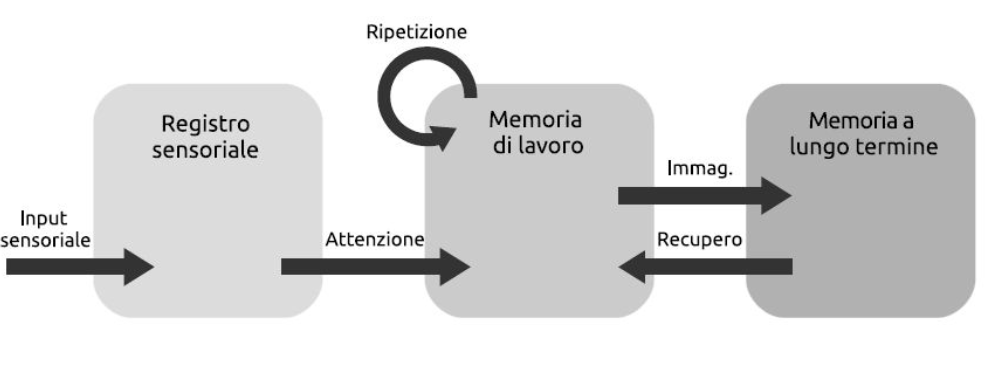
\includegraphics[scale = 0.4]{images/didattica della programmazione/Apprendimento.png}
\end{center}

\dfn{Registro sensoriale}{L'input sensoriale è ciò che viene acquisito dai 5 sensi.}

\nt{Nell'apprendimento l'input è solitamente l'udito o la vista.}

\dfn{Memoria a breve termine (o memoria di lavoro)}{Serve attenzione per passare dal registro sensoriale alla memoria di lavoro. Ha una capienza limitata in termini di spazio e tempo (circa 10 secondi, aumentabli con la ripetizione.}

\nt{Quando si sta imparando la memoria di lavoro è totalmente concentrata su un compito.}

\dfn{Memoria a lungo termine}{Ha capacità potenzialmente illimitate\footnote{Non esattamente}. Non si è coscenti di queste memorie che devono essere portate, ogni volta, nella memoria di lavoro.}

\dfn{Apprendimento}{L'apprendimento richiede che la conoscenza avviene solo quando il concetto passa dalla memoria a breve termine alla memoria a lungo termine.}

\nt{Se si "impara" una cosa, ma il giorno dopo non si riesce più a replicarla non si ha apprendimento.}

\section{La programmazione}

\dfn{Programmare}{La \newfancyglitter{programmazione} è una rappresentazione di base fatta di schemi\footnote{Problemi}, le soluzioni e le informazioni associate.}

\nt{Ciò che distingue un esperto da un principiante è la capacità di attingere a molti più schemi memorizzati nella memoria a lungo termine.}

\qs{}{Com'è possibile che l'uomo riesca a svolgere attività mentali complesse con una memoria di lavoro tanto limitata?}

\begin{itemize}
    \item Si apprende meglio quando la memoria di lavoro non è troppo vuota o troppo piena;
    \item Il carico cognitivo è legato alla memoria di lavoro;
    \item Il carico cognitivo può essere:
    \begin{enumerate}
        \item Intrinseco: imposto dal compito;
        \item Pertinente: usate per creare o modificare schemi, ma non indispensabile;
        \item Estraneo: inutile.
    \end{enumerate}
\end{itemize}

\nt{
\begin{itemize}
    \item Si deve mantenere un carico pertinente elevato;
    \item Se il carico intrinseco è elevato non si apprende\footnote{Ci si concentra sul problema, ma non sugli schemi};
    \item Se il carico cognitivo è basso ci si annoia;
    \item Se possibile conviene ridurre il carico cognitivo di compiti difficili.
\end{itemize}
}

\pagebreak

\section{Pattern}

\ex{Un abuso di pattern}{
\begin{center}
    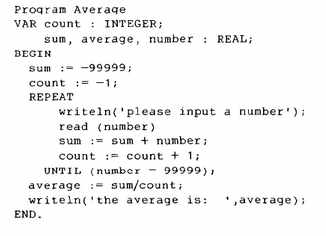
\includegraphics[scale = 0.7]{images/didattica della programmazione/Media.png}
\end{center}

Questo programma è stato scritto da uno studente che aveva intenzione di usare il pattern [Repeat Until] per risolvere il problema della media di una serie di input in cui il valore 99999 funge da guardia. Durante la progettazione lo studente si è trovato con il valore 99999 nella media (che ovviamente non deve essere incluso), motivo per cui ha dovuto inizializzare sum a -99999 (in questo modo i suoi valori si annullano)\footnote{Personalmente la ritengo una soluzione creativa, ma i docenti non sono dello stesso avviso}. Bisogna far capire allo studente che ci sono costrutti più indicati per risolvere questo problema, per esempio il while. Oltre a questo un errore è il count a - 1 che causa una divisione per 0 se si inserisce 99999 all'inizio, ma questo rappresenta un  problema successivo allo studio dei pattern\footnote{Casistica}. 
}

\ex{I pattern}{

\paragraph{Problema:} Si scriva un programma che trovi il minimo in un vettore non ordinato di dimensione nota, maggiore di 0, in cui ogni valore può raggiungere al massimo 99999.

\begin{enumerate}
    \item Input: vettore V[i], dimensione i;
    \item Si inizializza min a 99999, che andrà a trovare il minimo 
    \item Si effettua una [scansione elementare semplice] con l'indice i che viene decrementato a ogni iterazione;
    \item Durante la scansione si effettua una [Guarded-Action];
    \item Se la guardia è soddisfatta si aggiorna la variabile min;
    \item Se la guardia non è soddisfatta si continua finchè il ciclo non termina;
    \item Si stampa il valore min.
\end{enumerate}

}

\dfn{Possibile modo di definire un Pattern algoritmico}{

\begin{center}
    \begin{tabular}{ || p{10cm} ||}
    \hline\hline
    \textbf{Name:} il nome del pattern      
\\ \hline
        \textbf{Initial state:} l'input del programma
        \\
        \textbf{Goal:} l'obiettivo del programma
        \\
        \textbf{Algorithm:} l'algoritmo che risolve il problema
        \\
        \textbf{Remarks:} eventuali osservazioni importanti sul pattern e
        sul suo utilizzo
        \\\hline\hline
    \end{tabular}
\end{center}

}

\cor{Tipi di pattern}{
    \begin{itemize}
        \item [$\Rightarrow$] \textbf{Soluzione a un problema specifico:}
        non costituisce un vero pattern;
        \item [$\Rightarrow$] \textbf{Mezza soluzione - Mezzo pattern:}
        in parte rappresenta un pattern, ma è ancora troppo specifico;
        \item [$\Rightarrow$] \textbf{Quasi pattern:} si può generalizzare,
        ma lo pseudocodice è specifico;
        \item [$\Rightarrow$] \textbf{Pattern:} è generalizzato e lo
        pseudocodice è generico;
        \item [$\Rightarrow$] \textbf{Meta-pattern:} è un pattern che
        descrive un pattern\footnote{Troppo generico.}.
    \end{itemize}
}

\section{Il ruolo delle variabili}

\qs{}{Come viene usata una specifica variabile in un programma? Qual è
il suo ruolo?}

\nt{Si consiglia di non fare un elenco di tutti i vari tipi di utilizzo di
una variabile, ma di presentarli agli studenti quando si devono effettivamente
utilizzare in un programma.}

\dfn{Variabile - Valore fissato}{
    Una variabile assume il ruolo di valore fissato se non verrà mai modificato
    durante l'esecuzione del programma.
}

\nt{Un esempio è il valore di $\pi$.}

\dfn{Variabile - Contatore o indice}{
    Una variabile assume il ruolo di contatore o indice se viene usata per
    scorrere una successione di valori in modo sistematico.
}

\nt{Un esempio è l'indice di un vettore.}

\dfn{Variabile - Valore più recente}{
    Una variabile assume il ruolo di valore più recente se viene usata per
    memorizzare l'ultimo valore letto da un input.
}

\nt{Un esempio è la variabile che memorizza l'ultimo valore letto da un input.}

\dfn{Variabile - Valore più desiderato}{
    Una variabile assume il ruolo di valore più desiderato se viene usata per
    memorizzare il "miglior" valore incontrato fino a quel momento.
}

\nt{Un esempio è la variabile che memorizza il massimo di una successione.}

\subsection{Expert blind spot}

\qs{}{Si è certi che gli studenti siano in grado di riconoscere i ruoli delle variabili?}

\dfn{Expert blind spot}{
    L'expert blind spot è la difficoltà di un esperto di un argomento a
    comprendere le difficoltà che un principiante incontra quando si avvicina
    a quell'argomento.
}

\nt{Ricorda l'effetto Dunning-Kruger.}

\section{Comprensione del codice}

Ricapitolando, programmare vuol dire:

\begin{enumerate}
    \item formalizzare un problema e la sua soluzione;
    \item individuare un procedimento risolutivo;
    \item implementare il procedimento in un linguaggio di programmazione
    in modo che sia eseguibile.
\end{enumerate}

\dfn{Conoscenze}{
    \begin{itemize}
        \item [$\Rightarrow$] \textbf{Conoscenza sintattica:} conoscenza della
        sintassi del linguaggio di programmazione;
        \item [$\Rightarrow$] \textbf{Conoscenza concettuale:} conoscenza di come
        funzionano i costrutti del linguaggio di programmazione;
        \item [$\Rightarrow$] \textbf{Conoscenza strategica:} rappresenta la
        capacità di applicare le precedenti conoscenza per risolvere nuovi
        problemi.  
    \end{itemize}
}

\qs{}{Perchè nei corsi di introduzione alla programmazione si hanno spesso episodi di 
scarsa performance (big failure)?}

\begin{itemize}
    \item [$\Rightarrow$] Scarse competenze di problem solving;
    \item [$\Rightarrow$] Scarsa comprensione dei costrutti necessari per
    programmare;
    \item [$\Rightarrow$] Scarsa capacità di applicare le conoscenze assimilate.
\end{itemize}

\nt{Comprendere il codice e scrivere programmi sono due attività diverse.}

\dfn{Comprensione del codice}{
    La comprensione del codice è il processo cognitivo in cui un individuo costruisce
    una rappresentazione mentale di un programma.
}

\cor{Compito di comprensione del codice}{
    Il compito di comprensione del codice è un'attività tramite la quale si propone
    l'interazione con un pezzo di codice. Tramite questa interazione si costruisce
    una rappresentazione mentale del codice.
}

\mprop{Strategie nella didattica della programmazione}{
    \begin{itemize}
        \item [$\Rightarrow$] Insegnamento esplicito della conoscenza
        strategica;
        \item [$\Rightarrow$] Analisi delle specifiche;
        \item [$\Rightarrow$] Analisi del comportamento del codice; 
        \item [$\Rightarrow$] Tracciatura (simulazione del comportamento del
        programma);
        \item [$\Rightarrow$] Comprensione del codice ("spiega con parole tue");
        \item [$\Rightarrow$] Parsons problems (riordinare le righe di codice);
        \item [$\Rightarrow$] Refactoring di codice;
        \item [$\Rightarrow$] Adattamento di un programma a un compito simile;
        \item [$\Rightarrow$] Completamento di un programma;
        \item [$\Rightarrow$] Debugging;
        \item [$\Rightarrow$] Scrittura di codice.
    \end{itemize}
}

\subsection{Block Model}

\dfn{Block Model}{
    Il Block Model è un framework usato per classificare e analizzare vari aspetti
    della comprensione del codice.
}

\begin{figure}[!h]
    \centering
    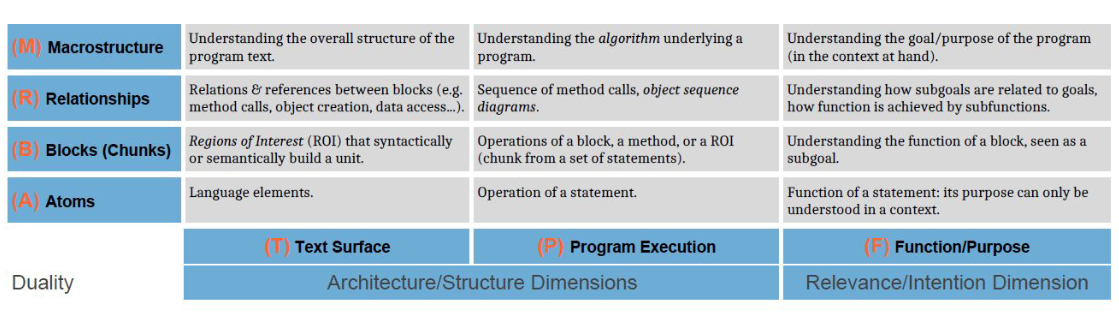
\includegraphics[scale = 0.4]{images/didattica della programmazione/Block Model.png}
    \caption{Block Model}
    \label{fig:my_label}
\end{figure}

\ex{Block Model}{
\begin{center}
    \begin{tabular}{ | p{10cm} | c | c |}
        \hline
        \textbf{\fancyglitter{Esercizio}} & \textbf{\fancyglitter{Comprensione}} & \textbf{\fancyglitter{Strategia}}      
\\ \hline\hline
    Indicare la struttura a blocchi di un programma
    & T
    & M\\\hline
    
    Determinare la presenza di codice ridondante
    & P
    & M\\ \hline
    
    Riassumere un programma in una breve frase
    & F
    & M\\\hline

    Identificare ogni assegnamento nel codice
    & T
    & A\\ \hline
    
    Determinare il valore di una variabile dopo l'esecuzione di un programma
    & P
    & A\\\hline
    
    Spiega lo scopo di un elemento di un programma
    & F
    & A\\ \hline
    
    Identifica lo scopo di una variabile
    & F
    & R\\\hline

    Identifica i blocchi di un programma
    & T
    & B\\ \hline    
    
    Completa il codice e un diagramma di flusso
    & P
    & B\\\hline
    
    Rifletti su un codice
    & T
    & R\\ \hline
    
    Parson's problem
    & P
    & R\\\hline
    
    Spiegare lo scopo di un programma
    & F
    & B\\ \hline
        \end{tabular}
    \end{center}
}

\subsection{Errori degli studenti}

\dfn{I distrattori}{
    I distrattori sono le risposte sbagliate che gli studenti danno più
    frequentemente nei test a risposta multipla. Esse sono impostate
    in modo da corrispondere a specifici errori concettuali.
}

\nt{In questi casi l'insegnate può facilmente individuare cosa lo studente non abbia capito\footnote{Assumendo che lo studente non abbia copiato o tirato a caso.}.}

\cor{5 livelli di risposte}{
    \begin{itemize}
        \item [$\Rightarrow$] \textbf{Prestructural:} la risposta dell'alunno
        è la meno sofisticata tra quelle possibili\footnote{È sintomo
        di un'idea sbagliata o di un preconcetto irrilevante.};
        \item [$\Rightarrow$] \textbf{Unistructural:} la risposta dell'alunno
        mostra una comprensione parziale del problema, una sorta di "congettura
        istruita";
        \item [$\Rightarrow$] \textbf{Multistructural:} la risposta dell'alunno
        rivela una consapevolezza di tutte le parti del problema, ma  non riesce
        a collegarle tra loro\footnote{"Not seeing the forest for the trees".};
        \item [$\Rightarrow$] \textbf{Relational:} la risposta dell'alunno
        rappresenta un'integrazione delle parti del problema;
        \item [$\Rightarrow$] \textbf{Extended abstract:} la risposta dell'alunno va
        al di là del problema immediato ed è collegata a un contesto più ampio;
    \end{itemize}
}

\dfn{Scaffolding}{
    Lo scaffolding è un processo di supporto che aiuta gli studenti:
    \begin{itemize}
        \item Ridurre il carico cognitivo;
        \item Fornire un modello di soluzione adeguato;
        \item Favorire lo sviluppo di una conoscenza strategica.
    \end{itemize}
}

\nt{Ovviamente lo scaffolding deve essere piano piano rimosso.}

\section{Approcci innovativi}

\subsection{PRIMM}

\dfn{PRIMM}{
    PRIMM è un framework per la progettazione di attività didattiche
    per l'insegnamento della programmazione comprendente le seguenti fasi:
    \begin{itemize}
        \item \textbf{Predizione:} gli studenti devono prevedere il
        comportamento di un programma;
        \item \textbf{Esecuzione:} gli studenti devono eseguire il programma
        e verificare la predizione;
        \item \textbf{Investigazione:} gli studenti devono correggere la
        predizione in caso di errore;
        \item \textbf{Modifica:} gli studenti devono modificare il programma
        in modo che si comporti in un modo diverso;
        \item \textbf{Risoluzione:} gli studenti devono risolvere un problema
        usando il programma.
    \end{itemize}

}

\subsection{POGIL}

\dfn{POGIL}{
    POGIL è un framework per la progettazione di attività didattiche
    per l'insegnamento della programmazione. Durante queste attività gli
    studenti attraversano un ciclo di esplorazione, concettualizzazione e
    applicazione.
    Gli studenti scoprono i concetti chiave e costruiscono la propria
    conoscenza attraverso l'interazione con i compagni e con il docente.
}

\subsection{NDL}

\dfn{NDL}{
    NDL (Necessity design learning) è un framework per la progettazione di attività didattiche
    per l'insegnamento della programmazione. Sostanzialmente si dà un problema
    risolvibile con un certo costrutto senza introdurlo. Successivamente,
    prima che lo studente si scoraggi, si introduce il costrutto.
}
